\documentclass[11pt]{article}
%\usepackage{amsfonts}
\usepackage{amsmath}
\usepackage{fancybox}%,times}
\usepackage{graphicx,psfrag,epsf}
%\usepackage{amsmath}
\usepackage{enumerate}
\usepackage{graphicx,psfrag}
\usepackage{multirow}
\usepackage{epsfig}
%\usepackage{rotating}
\usepackage{subfigure}
\usepackage{theorem}
\usepackage{natbib,psfrag}
\usepackage{tikz}
\usepackage{xcolor}
\usepackage{kotex}
\newcommand{\blind}{0}
\usepackage{graphicx}
\DeclareGraphicsExtensions{.pdf,.png,.jpg}

\addtolength{\oddsidemargin}{-.75in}%
\addtolength{\evensidemargin}{-.75in}%
\addtolength{\textwidth}{1.5in}%
\addtolength{\textheight}{1.3in}%
%\addtolength{\topmargin}{-.6in}%
\addtolength{\topmargin}{-.8in}%

%\theoremstyle{break}
\newtheorem{The}{Theorem}
\newtheorem{Def}{Definition}
\newtheorem{Pro}{Proposition}
\newtheorem{Lem}{Lemma}
\newtheorem{Cor}{Corollary}
\newtheorem{asp}{Assumption}


\renewcommand{\thefootnote}{\arabic{footnote}}
%\renewcommand{\thefootnote}{\alph{footnote}}
%\renewcommand{\thefootnote}{\roman{footnote}}
%\renewcommand{\thefootnote}{\fnsymbol{footnote}}

\begin{document}
	
	
	%\bibliographystyle{natbib}
	
	\newcommand{\Ito}{$It\hat{o}$'$s~Lemma$}
	
	\newcommand\ind{\stackrel{\rm ind}{\sim}}
	\newcommand\iid{\stackrel{\rm iid}{\sim}}
	\renewcommand\c{\mathbf{c}}
	\newcommand\y{\mathbf{y}}
	\newcommand\z{\mathbf{z}}
	\renewcommand\P{\mathbf{P}}
	\newcommand\W{\mathbf{W}}
	\newcommand\X{\mathbf{X}}
	\newcommand\Y{\mathbf{Y}}
	\newcommand\Z{\mathbf{Z}}
	\newcommand\J{{\cal J}}
	\newcommand\B{{\cal B}}
	\newcommand\K{{\cal K}}
	\newcommand\N{{\rm N}}
	\newcommand\bs{\boldsymbol}
	\newcommand\bth{\bs\theta}
	\newcommand\bbe{\bs\beta}
	\renewcommand\*{^\star}
	
	\def\spacingset#1{\renewcommand{\baselinestretch}%
		{#1}\small\normalsize} \spacingset{1}
	
	
	%%%%%%%%%%%%%%%%%%%%%%%%%%%%%%%%%%%%%%%%%%%%%%%%%%%%%%%%%%%%%%%%%%%%%%%%%%%%%%
	
	\bigskip
	\bigskip
	\bigskip
	\begin{center}
		{\LARGE\bf September 19, 2019 }
	\end{center}
	\medskip
	
	%\begin{abstract}
	%\end{abstract}
	
	%\noindent%
	%{\it Key Words:}  AECM algorithm; Astrophysical data analysis;
	%ECME algorithm; Incompatible Gibbs sampler; Marginal data
	%augmentation; Multiple imputation; Spectral analysis
	
	\spacingset{1.45}
	
	
	
	\section{Empirical Bayes}
	
	\begin{align*}
		Y|\beta,\sigma^2 ,\gamma &\sim N(Z\Gamma\beta , \sigma^2 I)\\
		\sigma^2 &\sim Inverse-Gamma(A,B)  \;\;\;\ A=0,\;B=0\\
		\beta_j &\sim N(0, \sigma_{\beta}^2)\\
		\gamma_j &\sim Bernoulli(\rho)
	\end{align*}
	
	We need to calculate the likelihood $p(y|\rho)$ and select the hyper parameter $\rho$ which maximize the likelihood
	
	by varational bayes approach we can find lower bound of $p(y|\rho)$
	
	\begin{align*}
	\log p(y|\rho) \ge \sigma_{\gamma} \int q(\beta,\sigma^2,\gamma) \log\left\{\frac{p(y,\beta,\sigma^2,\gamma)}{q(\beta,\sigma^2,\gamma)}\right\} d\beta d\sigma^2  = ELBO(\rho)
	\end{align*} 
	
	\begin{align*}
	ELBO(\rho) =& c -(A + \frac{n}{2}) \log(s) + \frac{1}{2}|\Sigma| - \frac{1}{\sigma_{\beta}^2} tr(\mu \mu' + \Sigma) \\
	& + \sum_{j=1}^{p} \left[ w_j \log\left(\frac{\rho}{w_j} + (1-w_j)\log\left( \frac{1-\rho}{1-w_j}\right)\right)\right]
	\end{align*}
	when variation distribution is
	\begin{align*}
	q(\beta) &\sim N(\mu,\Sigma)\\
	q(\sigma^2) &\sim Inverse-Gamma(A+n/2,s)\\
	q(\gamma_j) &\sim Bern(w_j) \;\;\; for \;\; j =1,\dots,p 
	\end{align*} 

	\begin{figure} [h]
		\centering
		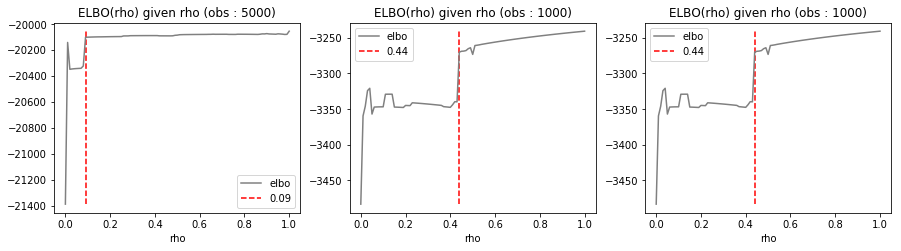
\includegraphics[width=1\linewidth]{output_28_0}
		\caption{ELBO($\rho$) plot by observation counts}
		\label{fig:output280}
	\end{figure}

	\begin{figure} [h]
		\centering
		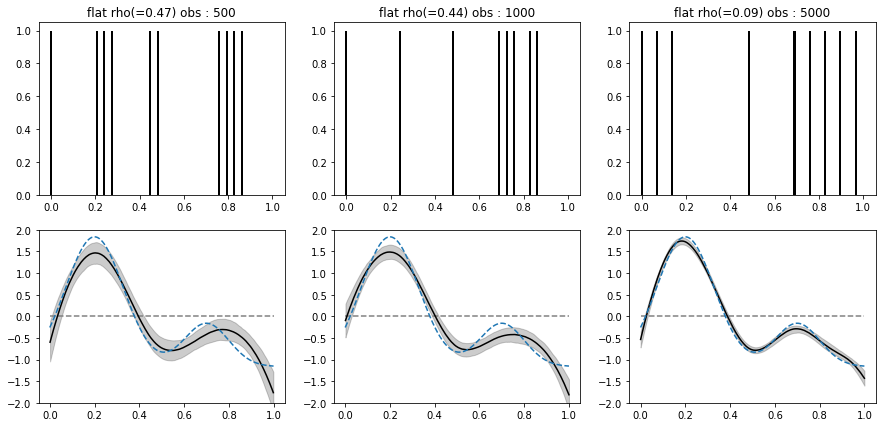
\includegraphics[width=1\linewidth]{output_40_0}
		\caption{Empirical Bayes with optiaml $\rho$}
		\label{fig:output400}
	\end{figure}
	\newpage
	\section{Hierarchical Bayes}
	\begin{align*}
		Y|\beta,\sigma^2 ,\gamma &\sim N(Z\Gamma\beta , \sigma^2 I)\\
		\sigma^2 &\sim Inverse-Gamma(A,B)  \;\;\;\ A=0,\;B=0\\
		\beta_j &\sim N(0, \sigma_{\beta}^2)\\
		\gamma_j &\sim Bernoulli(\rho)\\
		\rho &\sim Beta(C,D)
	\end{align*}
	\begin{figure} [h]
		\centering
		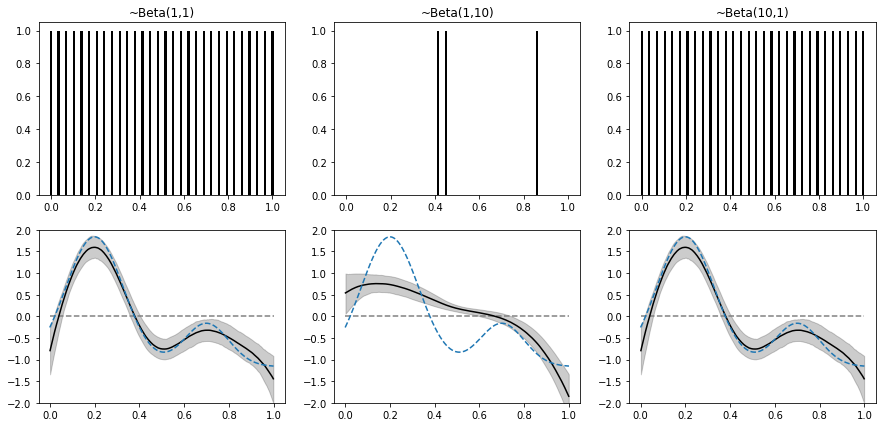
\includegraphics[width=1\linewidth]{output_35_1}
		\caption{Hierarchical model with obs=500, posterior mean is 0.72, 0.22, 0.78}
		\label{fig:output351}
	\end{figure}
	
	\begin{figure} [h]
		\centering
		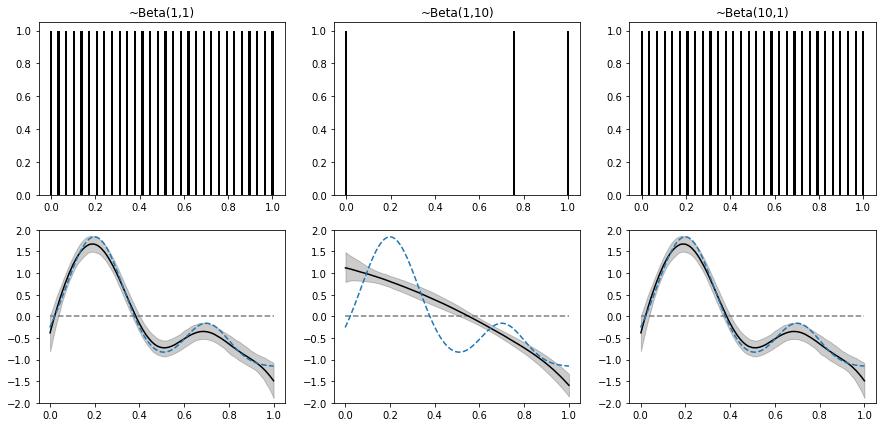
\includegraphics[width=1\linewidth]{output_36_1}
		\caption{Hierarchical model with obs=1000, posterior mean is 0.72, 0.22, 0.78}
		\label{fig:output351}
	\end{figure}
	\begin{figure} [h]
		\centering
		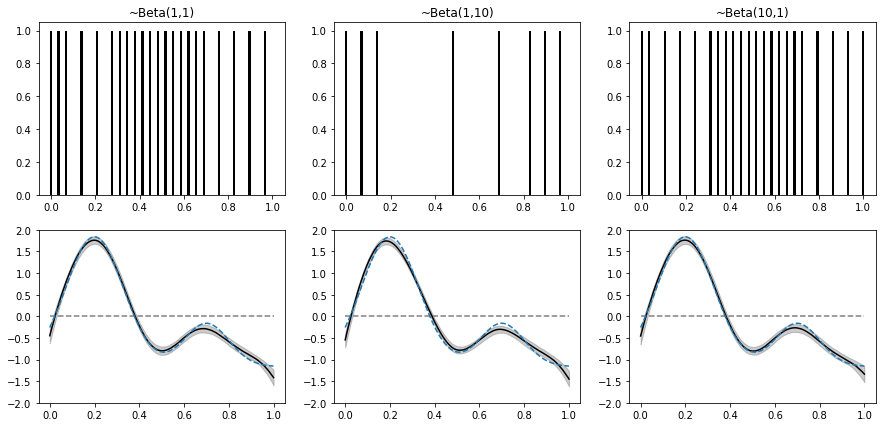
\includegraphics[width=1\linewidth]{output_37_1}
		\caption{Hierarchical model with obs=5000, posterior mean is 0.72, 0.22, 0.78}
		\label{fig:output351}
	\end{figure}
	
\end{document}